%% ma: L12-B04-0011
%% lop: 12
%% chuong: 1
%% bai: 4
%% dang: 12.4.11
%% loai: DS
%% muc: [NB, TH, VD, VDC]
%% dap_an: "SĐĐS"
%% nguon: "(NBV)-ĐỀ SỐ 14-MỖI NGÀY 1 ĐỀ THI 2025.pdf (D14, MỖI NGÀY 1 ĐỀ - Đề số 14), Phần II Câu 2"
%% kien_thuc: "Bài 1 (cực trị), Bài 2 (giá trị nhỏ nhất), Bài 4 (số nghiệm phương trình, tương giao); đặt ẩn phụ căn thức"
%% trang_thai: cho-duyet
%% ly_do: "Dạng mới 12.4.11 đề xuất, chờ giáo viên duyệt"
%% ghi_chu: "Kết luận gốc (a Sai, b Đúng, c Đúng, d Sai) đúng, nhưng lời giải gốc ý d) viết sai mẫu thức (t^2-4t+8 thay vì (t-3)^2+1); số đúng là 8 giá trị nguyên m = 1..8. Giữ phương án d) là 7 như đề gốc. Hình là bảng biến thiên dựng lại (đề không cho giá trị ở hai đầu)."
\begin{ex}
Cho hàm số $y=f(x)$ có bảng biến thiên như sau:
\begin{center}
\begin{tikzpicture}
  \tkzTabInit[lgt=1.2,espcl=2.4]{$x$/.8,$y'$/.8,$y$/2.4}{$-\infty$,$-2$,$1$,$3$,$+\infty$}
  \tkzTabLine{,-,0,+,0,-,0,+,}
  \tkzTabVar{+/$+\infty$,-/$-2$,+/$6$,-/$1$,+/$8$}
\end{tikzpicture}
\end{center}
\choiceTF
{Hàm số đã cho có hai điểm cực đại.}
{\True Giá trị nhỏ nhất của hàm số $y=f\left(\sqrt{x-3}+1\right)$ trên nửa khoảng $[3;+\infty)$ là $1$.}
{\True Phương trình $f(x)+x^2-6x=0$ có đúng hai nghiệm phân biệt lớn hơn $1$.}
{Có đúng $7$ số nguyên $m$ để phương trình $f\left(\sqrt{x-3}+1\right)+m\left(x+2-4\sqrt{x-3}\right)=10$ có hai nghiệm.}
\loigiai{a) $y'$ đổi dấu từ $+$ sang $-$ chỉ tại $x=1$ nên hàm số có đúng một điểm cực đại ($x=-2$ và $x=3$ là điểm cực tiểu). Sai.

b) Với $x\ge3$, đặt $t=\sqrt{x-3}+1$ thì $t$ nhận mọi giá trị trong $[1;+\infty)$. Trên $[1;+\infty)$, $f$ có giá trị nhỏ nhất là $f(3)=1$ (vì $f(1)=6$, $f$ giảm đến $f(3)=1$ rồi tăng). Đúng.

c) Xét $h(x)=f(x)+x^2-6x$ trên $(1;+\infty)$, $h'(x)=f'(x)+2x-6$. Trên $(1;3)$: $f'(x)<0$ và $2x-6<0$ nên $h$ nghịch biến, $h(1)=1>0$, $h(3)=-8<0$: đúng một nghiệm. Trên $(3;+\infty)$: $f'(x)>0$ và $2x-6>0$ nên $h$ đồng biến, $h(3)<0$ và $h(x)\to+\infty$: đúng một nghiệm. Vậy có đúng hai nghiệm lớn hơn $1$. Đúng.

d) Đặt $t=\sqrt{x-3}+1\ge1$ (mỗi $t$ ứng với đúng một $x$); khi đó $x+2-4\sqrt{x-3}=(t-3)^2+1$ và phương trình trở thành $m=g(t)=\dfrac{10-f(t)}{(t-3)^2+1}$, $t\ge1$.
Trên $[1;3]$: $10-f(t)$ tăng từ $4$ đến $9$, mẫu giảm từ $5$ xuống $1$ nên $g$ tăng từ $0{,}8$ đến $9$. Trên $[3;+\infty)$: $10-f(t)$ giảm từ $9$ đến $2$, mẫu tăng đến $+\infty$ nên $g$ giảm từ $9$ về $0$ (không đạt). Phương trình có hai nghiệm khi và chỉ khi $0{,}8\le m<9$, tức $m\in\{1;2;\dots;8\}$: có $8$ số nguyên, không phải $7$. Sai.}
\end{ex}
